% ============================================================
%  Section 3 — Dataset ewat_v3
% ============================================================

\section{Dataset ewat\_v3}
\label{sec:dataset}

Le dataset ewat\_v3 est issu d'une collecte expérimentale sur infrastructure réelle.
L'utilisation d'un cluster Kubernetes de production simulée — plutôt que d'un simulateur
ou d'un dataset public — est un choix délibéré : les couplages inter-services réels,
les bruits d'observabilité et les artefacts de timing (retards de scraping Prometheus,
buffers OTel) sont indispensables pour que le pipeline soit évaluable dans des conditions
représentatives du déploiement en production.

\subsection{Infrastructure expérimentale}
\label{sec:infra}

Le cluster \texttt{observit-cluster1} est un cluster RKE2 v1.32.7 composé de 9 nœuds
(8 Ready, 1 NotReady : \texttt{observit-cluster1-workers-58w74-mwxb2}, source du
16.7\,\% de NaN sur \texttt{disk\_io} pour le service \texttt{product-catalog}).
L'application hébergée est \emph{Online Boutique} de Google, une boutique en ligne
constituée de microservices hétérogènes (Go, Python, Java, Node.js) couvrant les services
\texttt{frontend}, \texttt{cart}, \texttt{load-generator}, \texttt{recommendation},
\texttt{ad} et \texttt{product-catalog}.

Les injections de pannes sont réalisées avec Chaos Mesh, un opérateur Kubernetes permettant
de définir des scénarios reproductibles sous forme de CRDs.
La stack d'observabilité combine Prometheus (métriques Kubernetes et applicatives) et un
OpenTelemetry Collector recevant les traces et logs applicatifs en OTLP gRPC.

\subsection{Protocole de collecte}
\label{sec:collect}

La collecte suit un protocole en trois phases :

\begin{enumerate}
  \item \textbf{Phase 1 — Enregistrement} (\texttt{scripts/record\_episode.py}) :
    injection d'un scénario Chaos Mesh, dump brut des métriques Prometheus
    et des spans OTel sur une fenêtre de $\approx 10$\,min
    ($T \approx 21$ steps à 30\,s/step).

  \item \textbf{Phase 2 — Construction des features}
    (\texttt{scripts/build\_features.py}) :
    extraction du signal $S(t) \in \mathbb{R}^{N \times 17}$, du graphe $G(t)$
    et des labels de régime depuis les dumps bruts.

  \item \textbf{Phase 3 — Assemblage} (\texttt{scripts/assemble\_dataset.py}) :
    split stratifié $209 / 45 / 45$ (train / val / test)
    garantissant la représentation de chaque scénario dans les trois splits.
\end{enumerate}

Le split stratifié assure qu'aucun scénario n'est absent du jeu de test, condition
nécessaire pour évaluer H3 par type de cluster. Le ratio 209/45/45 correspond
approximativement à un split 70/15/15, classique pour des datasets de taille limitée.

\subsection{Composition}
\label{sec:composition}

Le dataset \texttt{ewat\_v3} comprend \textbf{299 épisodes}
(300 collectés, 1 rejeté — \texttt{network\_loss\_018}, Loki 100\,\% NaN)
répartis sur 15 scénarios :

\begin{itemize}
  \item \textbf{4 drifts bénins} :
    \texttt{drift\_config\_change}, \texttt{drift\_rolling\_deploy},
    \texttt{drift\_scale\_up}, \texttt{drift\_traffic\_ramp}.
  \item \textbf{11 anomalies vraies} :
    \texttt{cpu\_starvation}, \texttt{crash}, \texttt{fail\_slow\_cpu},
    \texttt{fail\_slow\_latency}, \texttt{faulty\_deploy\_overlap},
    \texttt{intermittent\_error}, \texttt{memory\_pressure},
    \texttt{network\_loss}, \texttt{noisy\_neighbor}, \texttt{oom},
    \texttt{resource\_leak}.
\end{itemize}

Les 6 services instrumentés sont :
\texttt{frontend}, \texttt{cart}, \texttt{load-generator},
\texttt{recommendation}, \texttt{ad}, \texttt{product-catalog}.

Chaque scénario dispose de $\approx 20$ répétitions, réparties de façon équilibrée sur les
trois splits. Le scénario \texttt{faulty\_deploy\_overlap} est particulier : il représente
le régime $\theta_{\text{drift} \cap \text{anomaly}}$, avec un déploiement défectueux qui
déclenche simultanément un drift de distribution et une dégradation des SLOs.

\subsection{Qualité du signal}
\label{sec:quality}

\begin{figure}[h]
\centering
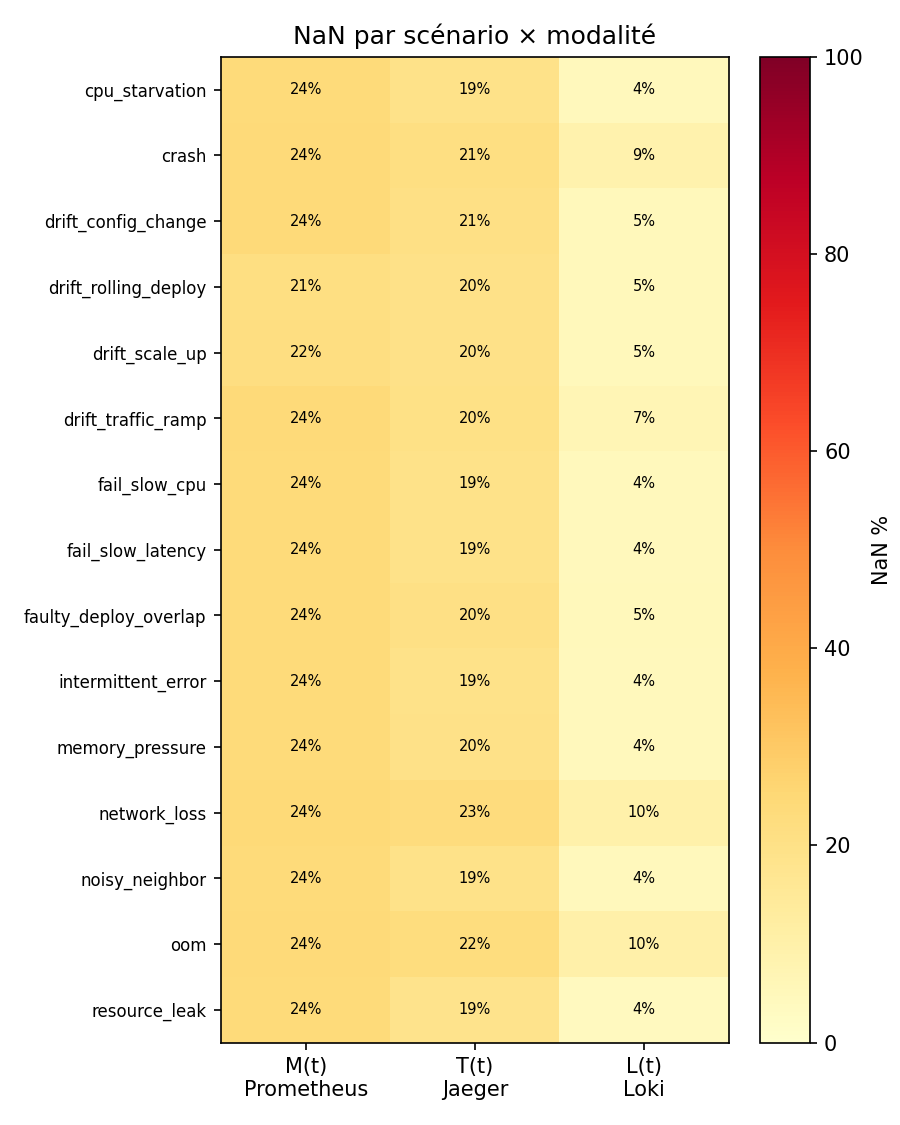
\includegraphics[width=0.82\linewidth]{figures/nan_heatmap.png}
\caption{Taux de NaN par feature et par scénario. \texttt{disk\_io} pour \texttt{product-catalog}
  présente systématiquement 16.7\,\% de NaN (nœud NotReady).}
\label{fig:nan_heatmap}
\end{figure}

\begin{figure}[h]
\centering
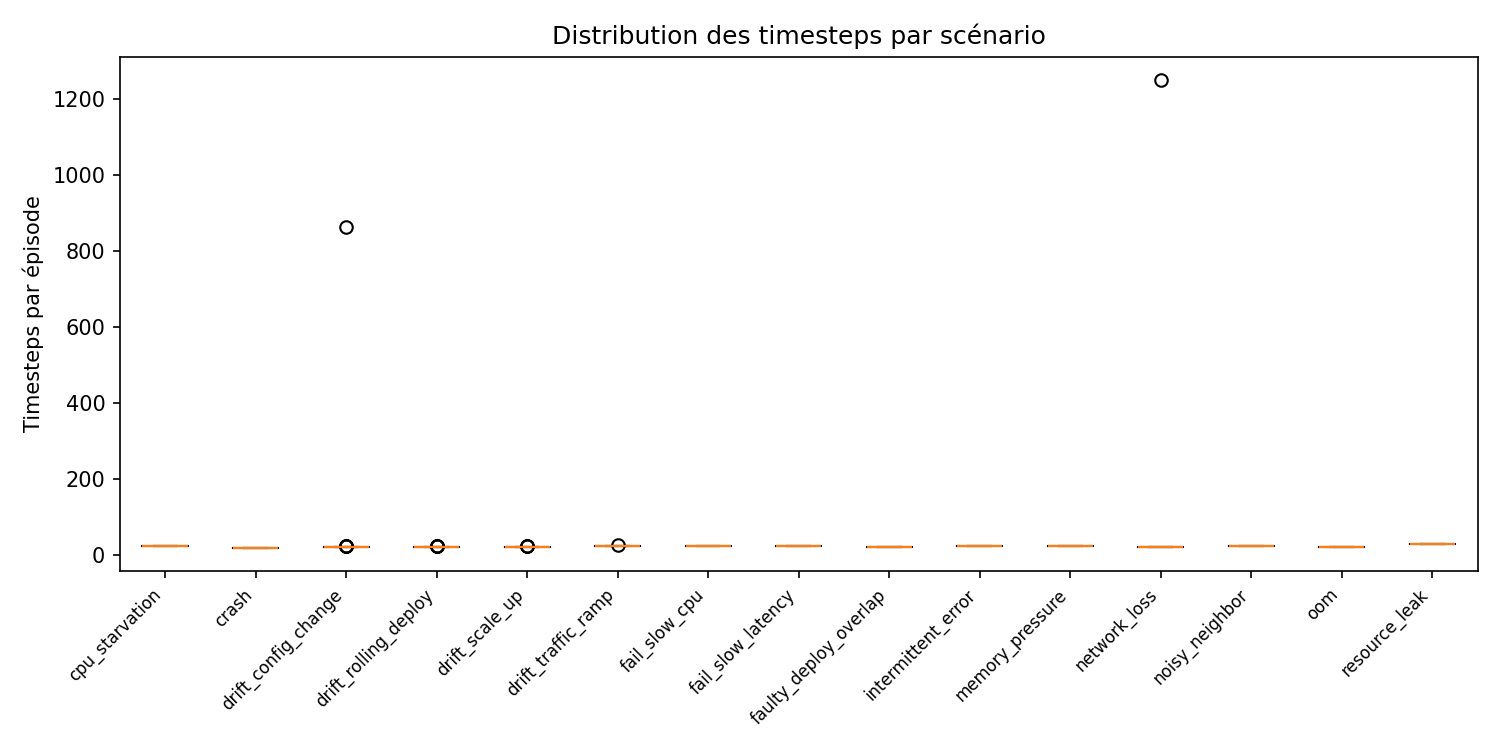
\includegraphics[width=0.72\linewidth]{figures/timesteps_boxplot.png}
\caption{Distribution de la longueur des épisodes par scénario ($T \approx 21$ steps,
  limitation L1).}
\label{fig:timesteps}
\end{figure}

\begin{table}[h]
\centering
\caption{Taux de valeurs manquantes par modalité.}
\label{tab:nan}
\begin{tabular}{lll}
\toprule
\textbf{Feature} & \textbf{NaN} & \textbf{Cause} \\
\midrule
cpu\_util, ram\_util, net\_sat, queue\_depth & 0\,\% & ✓ \\
latency\_p99, error\_rate\_http & 0\,\% & patchés depuis spans OTel \\
Traces (7–12) & 0\,\% & ✓ \\
Logs (13–16) & 0.4\,\% & résiduel irréductible \\
\textbf{disk\_io} & \textbf{16.7\,\%} & nœud NotReady (\texttt{product-catalog}) \\
\bottomrule
\end{tabular}
\end{table}

Le taux global de NaN est de $\approx 1.5$\,\%, quasi-entièrement concentré sur
\texttt{disk\_io} pour le service \texttt{product-catalog}. Ce NaN est structurel :
le nœud \texttt{observit-cluster1-workers-58w74-mwxb2} est resté en état NotReady
pendant l'intégralité de la collecte ewat\_v3, rendant les métriques de disque
indisponibles pour ce service. Les NaN sont imputés par zéro dans le pipeline
(valeur par défaut de la métrique en l'absence de scraping), ce qui sous-estime
l'importance réelle de \texttt{disk\_io} — confirmé par l'ablation LOO
(Section~\ref{sec:ablation_h3}, $\Delta = -0.088$).

\subsection{Limitations}
\label{sec:dataset_limitations}

\begin{description}
  \item[\textbf{L1 — Épisodes trop courts} ($\approx 21$ steps, $\approx 10.5$\,min).]
    La durée a été optimisée pour maximiser le nombre d'épisodes
    (trade-off débit vs.\ profondeur temporelle).
    Impact : insuffisant pour le mécanisme look-through (warm-up $\approx 8$ steps,
    confirmation $3$–$6$ steps), et lead time maximal observable limité à $\approx 5$\,min.
    Résolu dans ewat\_v4 ($\geq 40$ steps, durée $\geq 20$\,min par épisode).

  \item[\textbf{L2 — disk\_io 16.7\,\% NaN}.]
    L'ablation H3 (Section~\ref{sec:ablation_h3}) montre que \texttt{disk\_io} est
    la feature la plus critique pour les précurseurs ($\Delta = -0.088$),
    malgré ses valeurs manquantes — son importance réelle est probablement
    sous-estimée. Résolu dans ewat\_v4 par déploiement d'un OTel SDK applicatif
    permettant de collecter les métriques de disque indépendamment du nœud.
\end{description}
